\begin{landscape}
    \pagestyle{headings}
    \chapter{Schéma électrique}

    \begin{figure}[H]
        \centering
        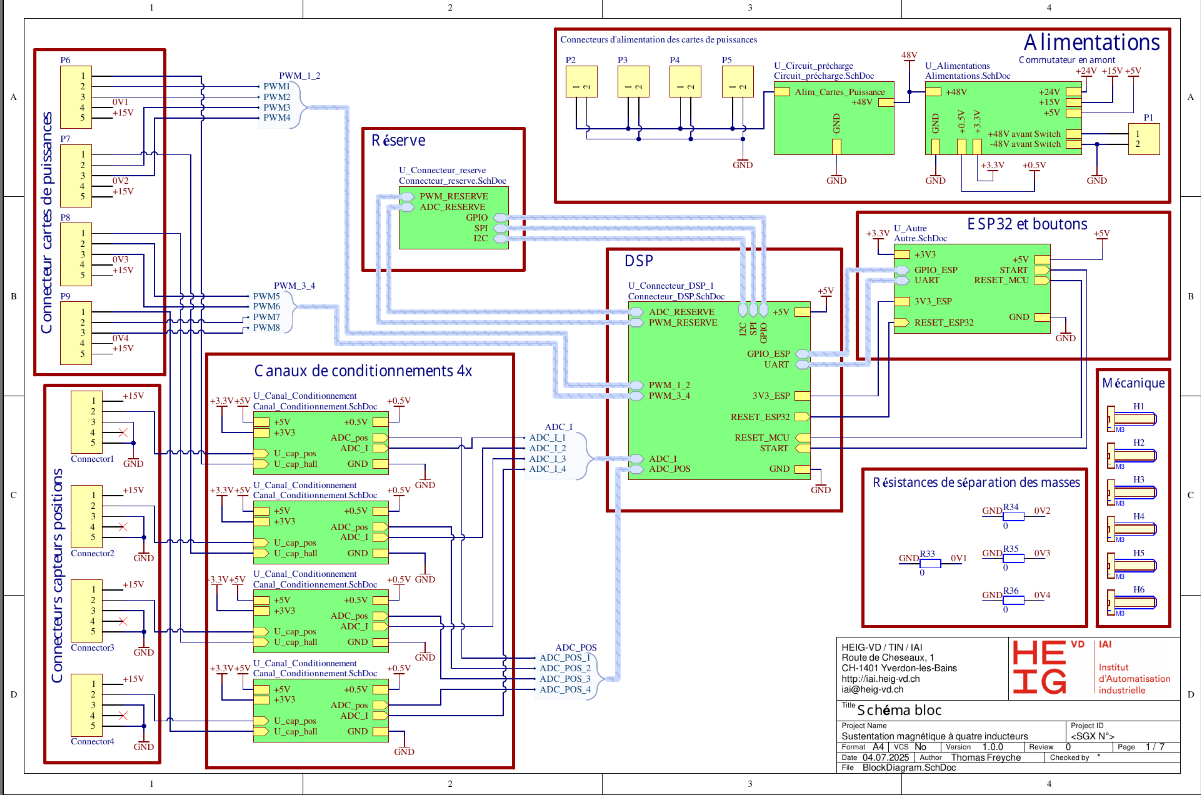
\includegraphics[height=\textheight, width=\linewidth, keepaspectratio, trim=5mm 5mm 1mm 0, clip]{Image/Chap.2/Scheme/SchemaComplet.png}
        \caption{Schéma électrique complet \cite{Freyche}}
    \end{figure}

    \begin{figure}[H]
        \centering
        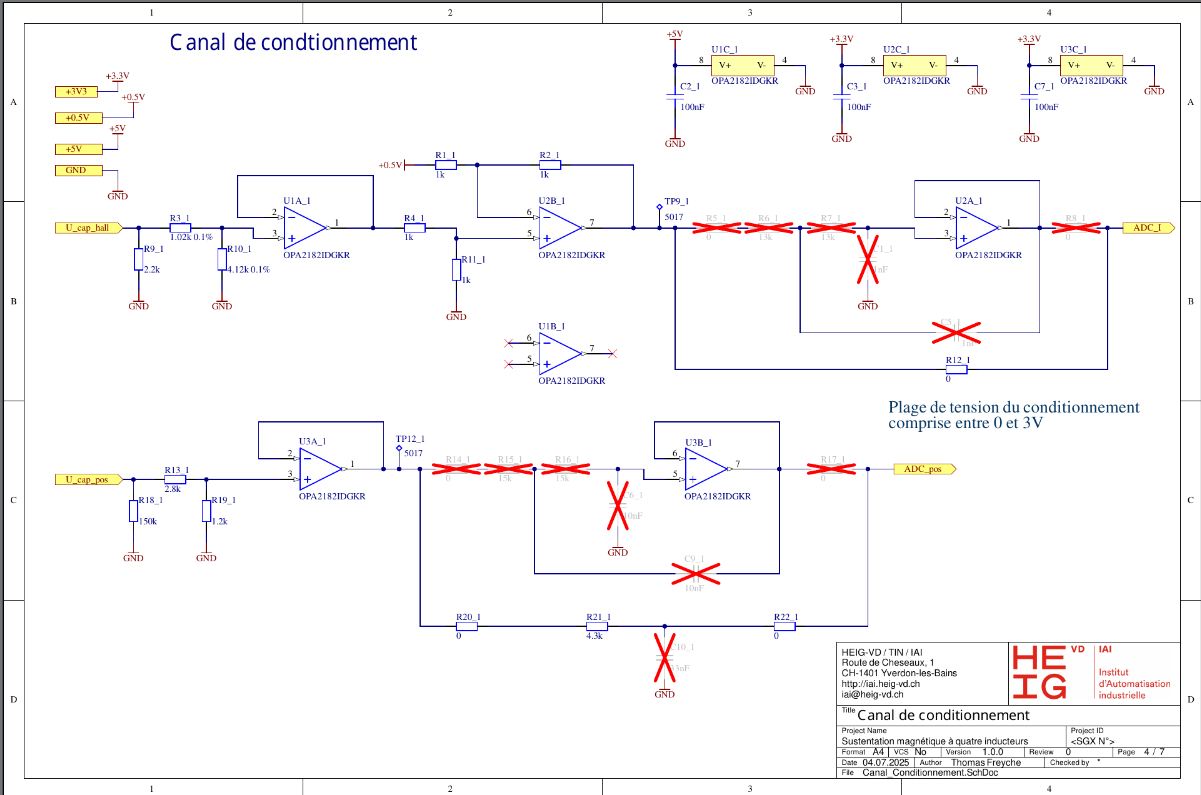
\includegraphics[height=\textheight, width=\linewidth, keepaspectratio, trim=5mm 0 1mm 5mm, clip]{Image/Chap.2/Scheme/DSP_Scheme.png}
        \caption{Connecteur pour la carte DSP \cite{Freyche}}
    \end{figure}

    \begin{figure}[H]
        \centering
        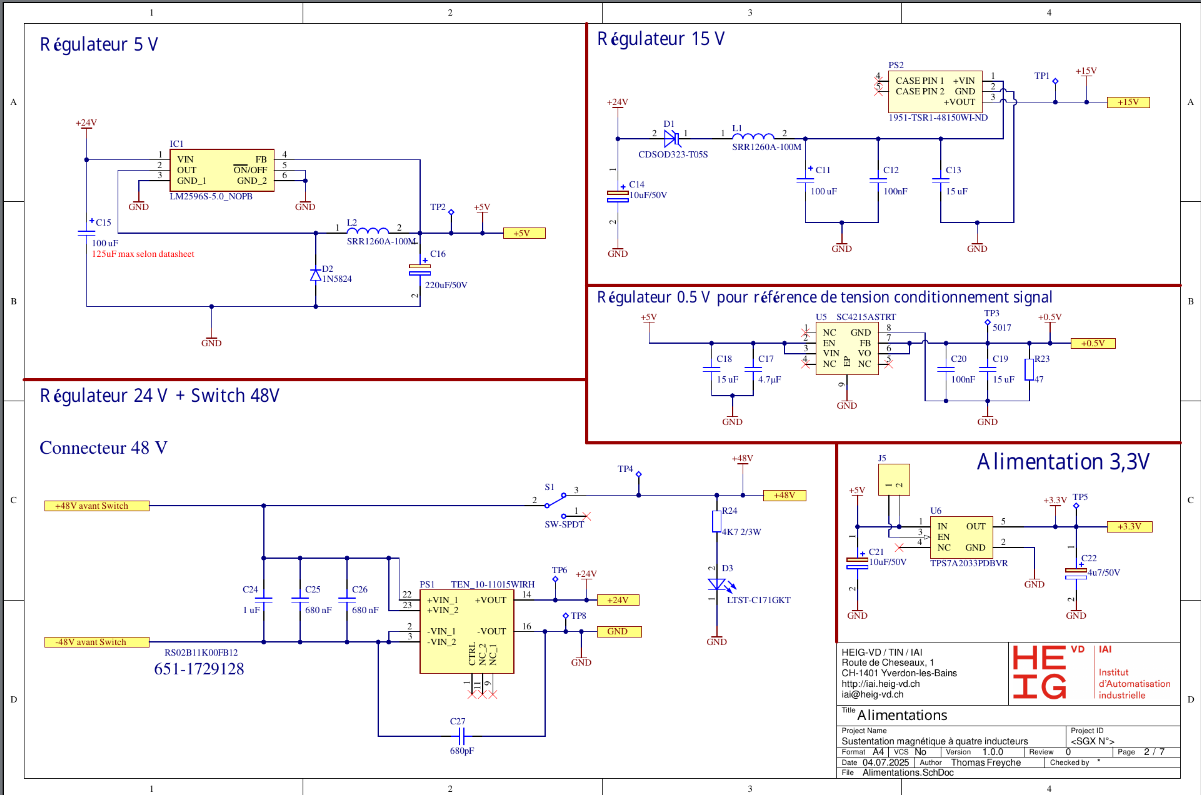
\includegraphics[height=\textheight, width=\linewidth, keepaspectratio, trim=5mm 0 1mm 5mm, clip]{Image/Chap.2/Scheme/ALimentation_Scheme.png}
        \caption{Canal de conditionnement \cite{Freyche}}
    \end{figure}

    \begin{figure}[H]
        \centering
        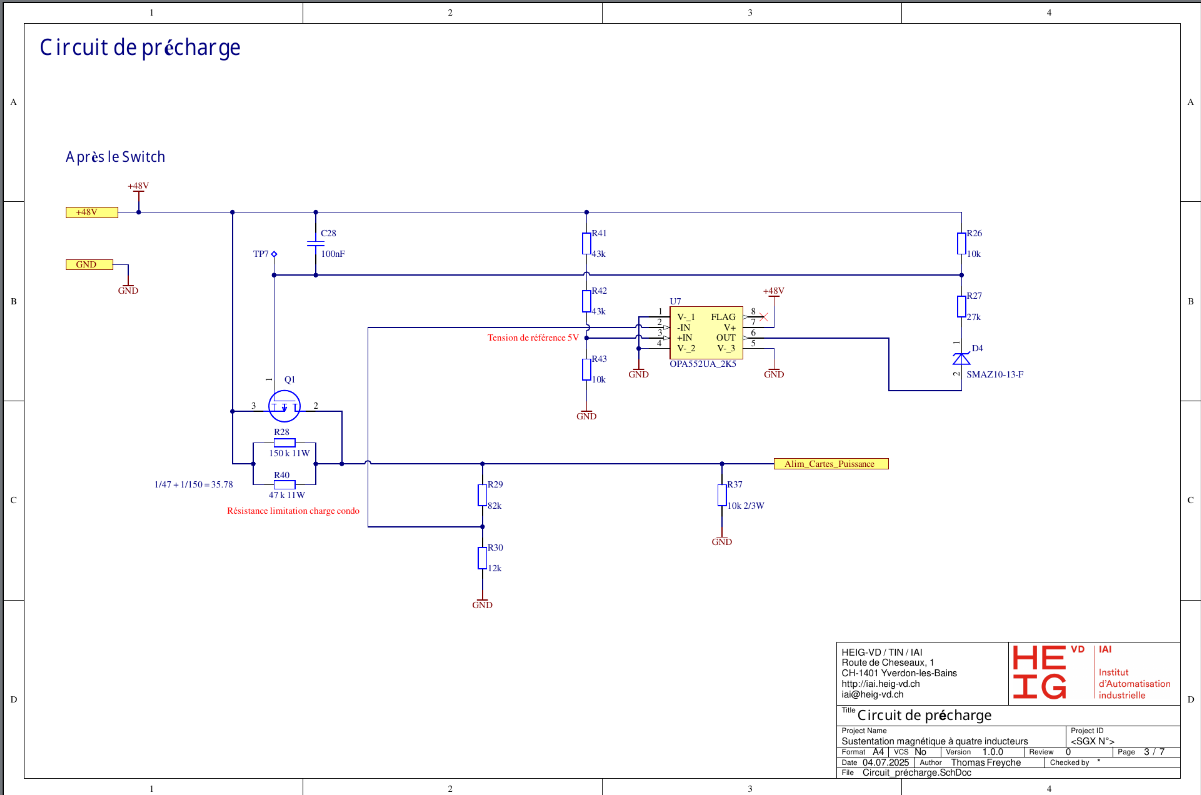
\includegraphics[height=\textheight, width=\linewidth, keepaspectratio, trim=5mm 0 1mm 5mm, clip]{Image/Chap.2/Scheme/Prech_Scheme.png}
        \caption{Circuit de précharge \cite{Freyche}}
    \end{figure}

    \begin{figure}[H]
        \centering
        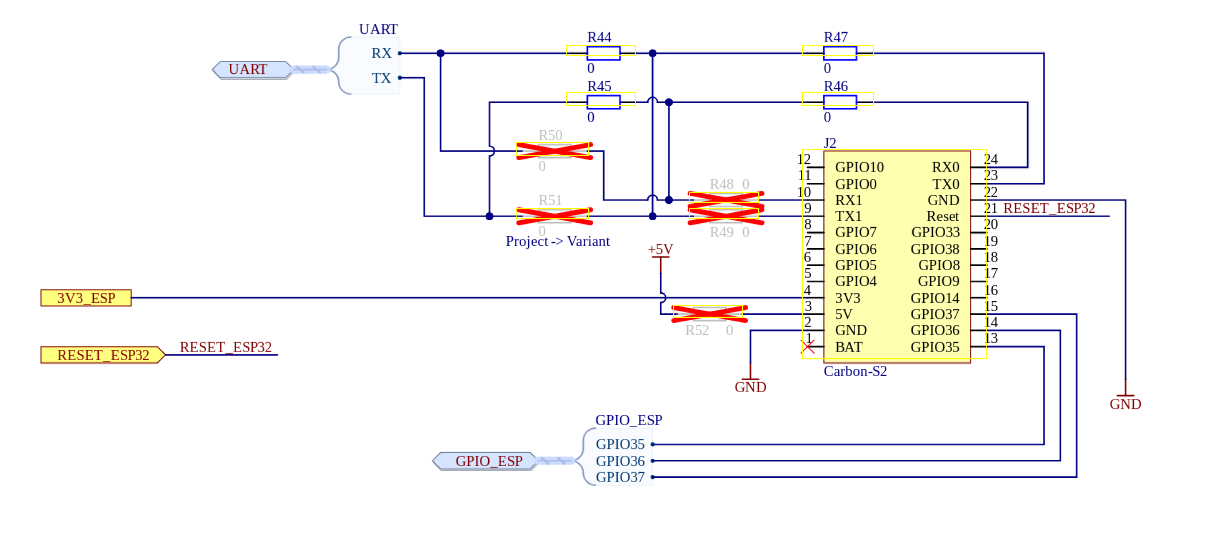
\includegraphics[height=\textheight, width=\linewidth, keepaspectratio, trim=5mm 0 1mm 0, clip]{Image/Chap.2/Scheme/ESP32_Scheme.png}
        \caption{Schéma de connexion de l'ESP32 \cite{Freyche}}
    \end{figure}
\end{landscape}